\documentclass[hidelinks]{article}

% ------------------------------------------------------------- Packages ---------------------------------------------------------------
\usepackage{lipsum}
\usepackage[margin=3cm,includefoot]{geometry}

% allows clickable references
\usepackage[hidelinks=true]{hyperref}

% math preamble
% \usepackage{mhchem} %if you want chemestry equation

% for graphic
\usepackage{graphicx}
\usepackage{float}

\usepackage{fancyhdr}
\pagestyle{fancy}
% clear head and foot (and create another foor)
\fancyhead{}
\fancyfoot{}
\fancyfoot[R]{\thepage\ }
% disable the line of the head and the footer
\renewcommand{\headrulewidth}{0pt}
\renewcommand{\footrulewidth}{0pt}

\begin{document}

% -------------------------------------------------------------- Title ---------------------------------------------------------------

\begin{titlepage}
	\begin{center}
            	\line(1,0){300} \\
        		[6mm]
	        	\huge{\bfseries Cybersecurity Visualization Mixed Reality} \\
        		[2mm]
	        	\line(1,0){300} \\
        		[1cm]
	        	\textsc {\LARGE Master's Thesis} \\
        		[0,5 cm]
	        	\textsc {\large Arts et Métiers ParisTech} \\
        		[0,5 cm]
	        	\textsc {\large University of Little Rock at Arkansas} \\
		[10cm]
	\end{center}
	
	\begin{flushright}
		\textsc {VERDIN-POL Gaétan \\
		July 20, 2018}
	\end{flushright}
\end{titlepage}




% ----------------------------------------------------------- Summary ---------------------------------------------------------------
\pagenumbering{roman}
\section *{Summary}
\addcontentsline{toc}{section}{\numberline{}Summary}
Summary or other section needed
\cleardoublepage

% ----------------------------------------------------------- Acknoledgements ---------------------------------------------------------------
\section *{Acknoledgements}
\addcontentsline{toc}{section}{\numberline{}Acknoledgements}
Thanks everybody
\cleardoublepage



% ----------------------------------------------------------- Table of contents ---------------------------------------------------------------

\tableofcontents
% remove the pagination for this page
\thispagestyle{empty}
\cleardoublepage


% -------------------------------------------------------------- Introduction ---------------------------------------------------------------

% set the counter to 1 after the introduction page
\pagenumbering{arabic}
\setcounter{page}{1}

\section{Introduction}\label{sec:intro}
Hey this is me and here come the introduction of my master's project \\
You know it \\

Here we have an indentation you know.
\lipsum[1]




% -------------------------------------------------------------- Section 1 ---------------------------------------------------------------

\newpage
\section{Section 1}
\lipsum[1] \\

% figure
\begin{figure}[H]
	\centering
	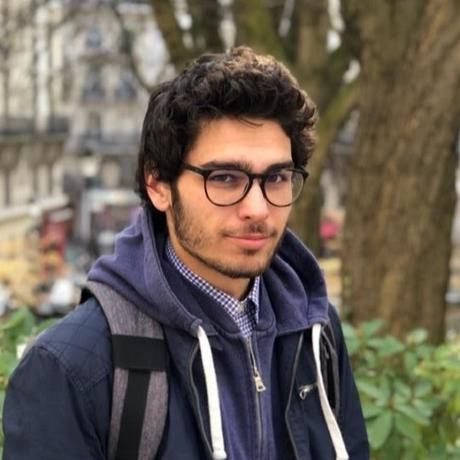
\includegraphics[height=3in]{/Users/gueguet57/Desktop/REPORT/latex_report/Images/profile_pic.jpeg}
	\caption[Optional caption]{Test capture} 
\end{figure}

\subsection{Subsection}
Ohla Que tal sub 1 yo on met ce qu'on veut hein tu coco, input ref here \cite{ref:ref_1}

\subsubsection{Sub-subsection}
This is a subsection of the subsection, you got it men \cite{ref:ref_2}

% list example
\begin{itemize}
	\item This is our first line
	\item Hello World
	\begin{itemize}
		\item list item iside a list
		\item you got it
	\end{itemize}
	\item It's again me
\end{itemize} 

% math equation
You can write math in LaTeX $E = mc^2$ or like this $$PV = NRT$$

We can use symbolus in our formulas

$$-\frac{\hbar^2}{2m} \frac{d^2\Psi}{dx^2} = 2 $$

$$ d = v_it + \frac{1}{2} \cdot ar^2$$

Brackets : 
$$\left(    \frac{1}{2}.    \right)   \cdot 2 = 1 $$

% table example
\begin{table}[H]
	\centering
	\caption[Caption for this table]{Local cap with ref}
	\begin{tabular}{ l c r}
		\bfseries{Date} & In tree? & Raining? \\ \hline
		April 26 & Yes & Yes \\
		June 7 & Yes & No \\
	\end{tabular}
\end{table}
	
\cleardoublepage
	
% -------------------------------------------------------------- Bibliographie ref ---------------------------------------------------------------
\bibliographystyle{IEEEtran}
\bibliography{/Users/gueguet57/Desktop/REPORT/latex_report/ref/report_ref.bib}
\addcontentsline{toc}{section}{\numberline{}References}
\cleardoublepage



% -------------------------------------------------------------- Appendix ---------------------------------------------------------------
\appendix
\section {Annexes}
This is an index
























\end{document}
